\documentclass[border=4pt]{standalone}
\usepackage[utf8]{inputenc}
\usepackage[T1]{fontenc}
\usepackage{amsmath,amssymb}
\usepackage[table]{xcolor}
\usepackage{tikz}
\usetikzlibrary{positioning,fit,calc,arrows.meta,shapes.geometric,decorations.pathreplacing,backgrounds}
\usepackage{pgfplots}
\pgfplotsset{compat=1.17}
\definecolor{stellantis}{RGB}{26,58,92}
\definecolor{sectionblue}{RGB}{44,95,138}
\definecolor{ddbrown}{RGB}{180,100,30}
\definecolor{ddbrownlight}{RGB}{255,243,230}
\begin{document}
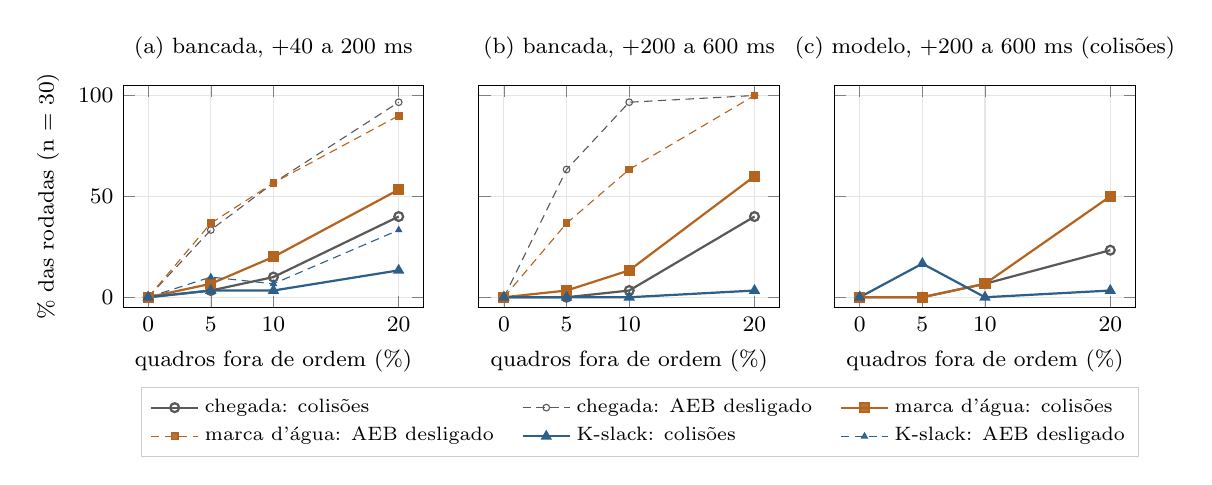
\begin{tikzpicture}
\begin{axis}[/pgf/number format/use comma, /pgf/number format/1000 sep={}, width=5.4cm, height=4.4cm, grid=major, grid style={gray!20}, tick label style={font=\footnotesize},
label style={font=\footnotesize}, legend style={font=\scriptsize, draw=gray!40, fill=white, fill opacity=0.9, text opacity=1},
xlabel={quadros fora de ordem (\%)}, xtick={0,5,10,20}, name=a, ylabel={\% das rodadas (n = 30)}, ymin=-5, ymax=105, title={\footnotesize (a) bancada, +40 a 200 ms}, legend columns=3, legend cell align=left, legend style={at={(1.72,-0.36)}, anchor=north, /tikz/every even column/.append style={column sep=8pt}}]
\addplot[color=gray!70!black, mark=o, mark size=1.6pt, thick] coordinates {(0,0.00) (5,3.33) (10,10.00) (20,40.00)};\addlegendentry{chegada: colisões}
\addplot[color=gray!70!black, mark=o, mark size=1.2pt, densely dashed, mark options={solid}] coordinates {(0,0.00) (5,33.33) (10,56.67) (20,96.67)};\addlegendentry{chegada: AEB desligado}
\addplot[color=ddbrown, mark=square*, mark size=1.6pt, thick] coordinates {(0,0.00) (5,6.67) (10,20.00) (20,53.33)};\addlegendentry{marca d'água: colisões}
\addplot[color=ddbrown, mark=square*, mark size=1.2pt, densely dashed, mark options={solid}] coordinates {(0,0.00) (5,36.67) (10,56.67) (20,90.00)};\addlegendentry{marca d'água: AEB desligado}
\addplot[color=sectionblue, mark=triangle*, mark size=1.6pt, thick] coordinates {(0,0.00) (5,3.33) (10,3.33) (20,13.33)};\addlegendentry{K-slack: colisões}
\addplot[color=sectionblue, mark=triangle*, mark size=1.2pt, densely dashed, mark options={solid}] coordinates {(0,0.00) (5,10.00) (10,6.67) (20,33.33)};\addlegendentry{K-slack: AEB desligado}
\end{axis}
\begin{axis}[/pgf/number format/use comma, /pgf/number format/1000 sep={}, width=5.4cm, height=4.4cm, grid=major, grid style={gray!20}, tick label style={font=\footnotesize},
label style={font=\footnotesize}, legend style={font=\scriptsize, draw=gray!40, fill=white, fill opacity=0.9, text opacity=1},
xlabel={quadros fora de ordem (\%)}, xtick={0,5,10,20}, at={(a.east)}, anchor=west, xshift=0.7cm, name=b, yticklabels={}, ymin=-5, ymax=105, title={\footnotesize (b) bancada, +200 a 600 ms}]
\addplot[color=gray!70!black, mark=o, mark size=1.6pt, thick] coordinates {(0,0.00) (5,0.00) (10,3.33) (20,40.00)};
\addplot[color=gray!70!black, mark=o, mark size=1.2pt, densely dashed, mark options={solid}] coordinates {(0,0.00) (5,63.33) (10,96.67) (20,100.00)};
\addplot[color=ddbrown, mark=square*, mark size=1.6pt, thick] coordinates {(0,0.00) (5,3.33) (10,13.33) (20,60.00)};
\addplot[color=ddbrown, mark=square*, mark size=1.2pt, densely dashed, mark options={solid}] coordinates {(0,0.00) (5,36.67) (10,63.33) (20,100.00)};
\addplot[color=sectionblue, mark=triangle*, mark size=1.6pt, thick] coordinates {(0,0.00) (5,0.00) (10,0.00) (20,3.33)};
\addplot[color=sectionblue, mark=triangle*, mark size=1.2pt, densely dashed, mark options={solid}] coordinates {(0,0.00) (5,0.00) (10,0.00) (20,3.33)};
\end{axis}
\begin{axis}[/pgf/number format/use comma, /pgf/number format/1000 sep={}, width=5.4cm, height=4.4cm, grid=major, grid style={gray!20}, tick label style={font=\footnotesize},
label style={font=\footnotesize}, legend style={font=\scriptsize, draw=gray!40, fill=white, fill opacity=0.9, text opacity=1},
xlabel={quadros fora de ordem (\%)}, xtick={0,5,10,20}, at={(b.east)}, anchor=west, xshift=0.7cm, yticklabels={}, ymin=-5, ymax=105, title={\footnotesize (c) modelo, +200 a 600 ms (colisões)}]
\addplot[color=gray!70!black, mark=o, mark size=1.6pt, thick] coordinates {(0,0.00) (5,0.00) (10,6.67) (20,23.33)};
\addplot[color=ddbrown, mark=square*, mark size=1.6pt, thick] coordinates {(0,0.00) (5,0.00) (10,6.67) (20,50.00)};
\addplot[color=sectionblue, mark=triangle*, mark size=1.6pt, thick] coordinates {(0,0.00) (5,16.67) (10,0.00) (20,3.33)};
\end{axis}
\end{tikzpicture}
\end{document}
